\newpage

\subsection{Einbindung und Konfiguration der Plugins}
\label{plugins}
Bei der Installation von Munin wird bereits eine Sammlung von Plugins mitgeliefert.
%Munin bringt bereits eine Sammlung von Plugins bei der Installation mit.
Diese befinden sich in einem Bibliotheksverzeichnis.
Wenn diese Plugins verwendet werden sollen um einen Node zu überwachen, müssen sie in einem Service-Verzeichnis verlinkt sein, damit der Daemon \pictext{munin-node} darauf zugreifen kann.
Dieser Daemon muss sich auf dem zu überwachenden Host befinden und dient als "`Agent"' für den Munin-Master, da der Daemon auf seinem Port nach Aufforderungen durch den Master lauscht.
Ein solcher Daemon ist für Linux und für Windows verfügbar, wobei der für Windows weniger Funktionen bietet.
Die einzelnen Tests laufen auf den Nodes; unabhängig von der Abfrage des Masters.
Wenn der Master die aktuellen Daten nicht abholt, wird dieser Datenbestand durch die neuen Informationen ausgetauscht und bei der nächsten Anfrage an den Master gesendet.

Auf den Graphen im Webinterface wird dieser Zeitraum als Lücke dargestellt, siehe Abbildung \ref{gap}.

\begin{figure}[ht]
	\centering
	   \fbox{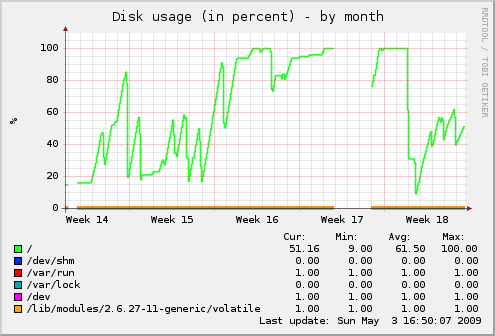
\includegraphics[width=0.852\textwidth]{bilder/gap.png}}
		\caption{Fehlende Messwerte werden als Lücke dargestellt}
		\label{gap}
\end{figure}

Der \pictext{munin-node}-Daemon kannn so konfiguriert werden, dass er nur auf Anfragen von einer bestimmten IP reagiert, einen anderen Port verwendet oder nur auf einer bestimmten IP lauscht.

Damit der Daemon weiß, welche Daten er liefern muss, wird das zuvor erwähnte Service-Verzeichnis verwendet.
Hier werden Verlinkungen zu den eigentlichen Plugins gespeichert.
Eine beispielhafte Verlinkung wird in Abbildung \ref{lns} gezeigt.

\begin{figure}[ht]
	\centering
	   \fbox{
\includegraphics[width=0.85\textwidth]{bilder/lns.png}}
		\caption{Beispielhafte Verlinkung eines Munin-Plugins}
		\label{lns}
\end{figure}

\subsubsection{Wildcard-Plugins}
\label{wildcard}
Falls der Name des Plugins mit einem Unterstrich endet, handelt es sich um ein sogenanntes \textit{Wildcard}-Plugin.
Alle Plugins dieser Kategorie erwarten in der Bezeichnung des Links spezifische Parameter für die Ausführung der Tests.

Beispielsweise verwendet das zuvor verwendete Plugin \textit{ping\_} als Parameter den Namen oder die IP-Adresse des anzupingenden Hosts.
Die Verlinkung aus dem Bibliotheksverzeichnis in das Service-Verzeichnis würde dann folgendermaßen ausschauen:
\begin{figure}[ht]
	\centering
	   \fbox{
\includegraphics[width=0.85\textwidth]{bilder/lnw.png}}
		\caption{Beispielhafte Verlinkung eines Wildcard-Plugins}
		\label{lnw}
\end{figure}

Hier wird der Host \textit{unilabad} angepingt und die Daten auf dem Master gespeichert um später in einem Graphen visualisiert zu werden.

\newpage

\subsubsection{SNMP-Plugins}
Es ist auch möglich Informationen über den zu überwachenden Host in Erfahrung zu bringen, ohne, dass ein \pictext{munin-node}-Daemon auf dem Host installiert ist.
Dies wird durch das Simple Network Management Protocol (SNMP) realisiert.
Durch SNMP kann auf die strukturierte Datenhaltung der MIB in den entfernten Netzwerkknoten zugegriffen werden.
\begin{quote}"`Die Management Information Base (MIB) dient als SNMP-Informations-struktur und besteht aus einem hierarchischen, aus Zahlen aufgebauten Namensraum. Ähnliche Struktur wie andere hierarchische Verzeichnisdiensten wie DNS oder LDAP."'\end{quote}
\begin{flushright}
Quelle: \cite{Barth08} S.233
\end{flushright}

Die MIB-Struktur ist folgendermaßen aufgebaut:

\begin{figure}[ht]
	\centering
	   \fbox{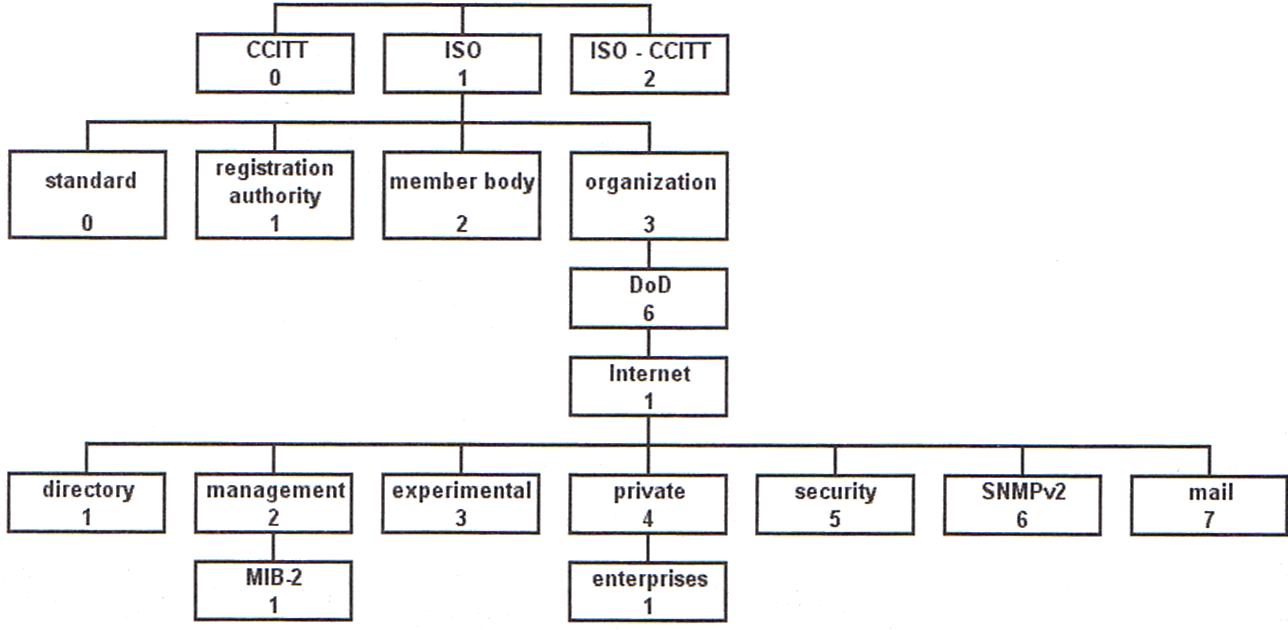
\includegraphics[width=0.95\textwidth]{bilder/mib.png}}
		\caption[Struktur der Management Information Base (MIB)]{Struktur der Management Information Base (MIB)\protect\footnotemark}
		\label{munin-mib}
\end{figure}
\footnotetext{Quelle: \cite{Mu08} S. 156}
Dadurch können die SNMP-Plugins den gewünschten Wert über das Netzwerk abfragen, ohne, dass ein lokal auf dem Munin-Node installiertes Programm notwendig ist.

\newpage

Einen beispielhaften Zugriff auf SNMP-fähige Geräte wird in Abbildung \ref{munin-snmp} gezeigt.

\begin{figure}[ht]
	\centering
	   \fbox{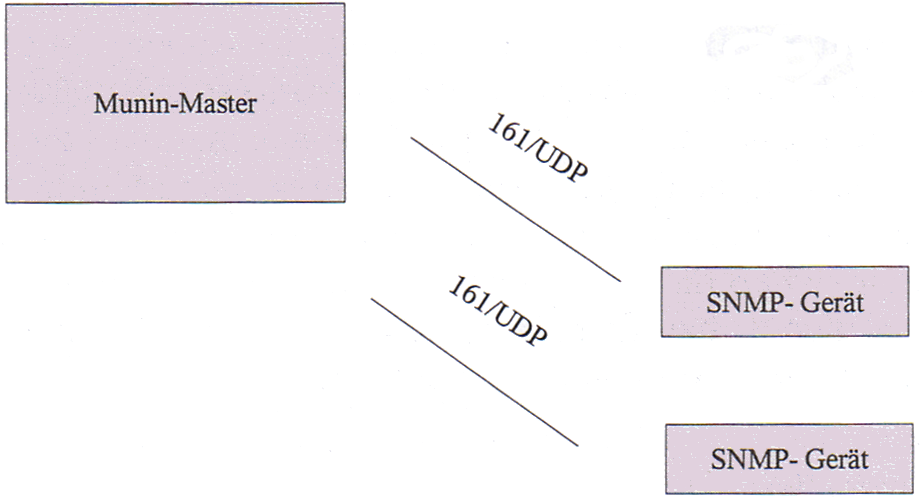
\includegraphics[width=0.85\textwidth]{bilder/snmp.png}}
		\caption[Beispielhafter Zugriff auf SNMP-fähige Geräte]{Beispielhafter Zugriff auf SNMP-fähige Geräte\protect\footnotemark}
		\label{munin-snmp}
\end{figure}
\footnotetext{Quelle: \cite{Mu08} S. 156}

Munin verwendet für SNMP-Plugins eine besondere Namenskonvention.
Alle Plugins dieser Art besitzen den Präfix \textit{snmp\_} auf den die IP-Adresse des SNMP-fähigen Gerätes folgt.
Im folgenden Beispiel wird die Speicherplatzauslastung eines entfernten Knotens überwacht.

\begin{figure}[ht]
	\centering
	   \fbox{
\includegraphics[width=0.85\textwidth]{bilder/snmp-simple.png}}
		\caption{Beispielhafte Verlinkung eines SNMP-Plugins}
		\label{snmp-simple}
\end{figure}

Auch bei diesen SNMP-Plugins gibt es Wildcard-Plugins.
Dabei wird als Suffix im unteren Beispiel der zweite Netzwerkport eines SNMP-fähigen Switches nach Paketfehler abgefragt.

\begin{figure}[ht]
	\centering
	   \fbox{
\includegraphics[width=0.85\textwidth]{bilder/snmp-complex.png}}
		\caption{Beispielhafte Verlinkung eines Wildcard-SNMP-Plugins}
		\label{snmp-complex}
\end{figure}

\newpage

Munin liefert unter anderem folgende SNMP-Plugins mit:

\begin{itemize}
\item \textit{snmp\_\_df} überwacht die Plattenbelegung.
\item \textit{snmp\_\_if\_} ermittelt den Netzwerkdurchsatz.
\item \textit{snmp\_\_if\_err\_} zählt die Paketfehler im Netzwerk.
\item \textit{snmp\_\_sensors\_\_fan} ermittelt die Lüfterdrehzahl.
\item \textit{snmp\_\_load} überwacht die Systemlast.
\item \textit{snmp\_\_processes} ermittelt die Anzahl der laufenden Prozesse.
\item \textit{snmp\_\_users} ermittelt die Anzahl der eingeloggten Benutzer.
\end{itemize}